\documentclass[journal=jacsat,manuscript=article]{achemso}
\usepackage[version=3]{mhchem}
\usepackage{amsmath}
\usepackage{ctex}
\usepackage{longtable}
\usepackage{booktabs}
\newcommand*\mycommand[1]{\texttt{\emph{#1}}}
\providecommand{\tightlist}{%
  \setlength{\itemsep}{0pt}\setlength{\parskip}{0pt}}
\author{蓝海}
\altaffiliation{我们认真科学分析金融的规律}
\email{lh_loki@163.com}
\phone{13127900572}
\author{彭莉}


\keywords{成长,学习型}

\title[王培]{王培简评\footnote{详尽的数据分析与记录请联系作者索取《基金管理人分析技术文档》}}
\makeatletter
\ifxetex
  \usepackage[setpagesize=false, % page size defined by xetex
              unicode=false, % unicode breaks when used with xetex
              xetex]{hyperref}
\else
  \usepackage[unicode=true]{hyperref}
\fi
\hypersetup{breaklinks=true,
            bookmarks=true,
            pdfauthor={},
            pdftitle={},
            colorlinks=true,
            urlcolor=blue,
            linkcolor=magenta,
            pdfborder={0 0 0}}
\urlstyle{same}  % don't use monospace font for urls
% pandoc header

\begin{document}
\begin{abstract}
王培是市场上成长股投资的明星。在10年的证券行业从业经历中,以基金经理人的身份长期管理多只偏股混合型基金,取得了不俗的投资收益。

基于公开信息分析,我们认为王培是从典型的成长股、相对集中型投资者逐渐转变为以成长价值为投资体系的基金管理人,体现了很强的适应市场的能力和学习总结的能力。其具备较强的选股能力和不太显著的行业配置能力,长期保持积极的主动投资。无明显的交易风格。
\end{abstract}
\begin{figure}[htbp]
\centering
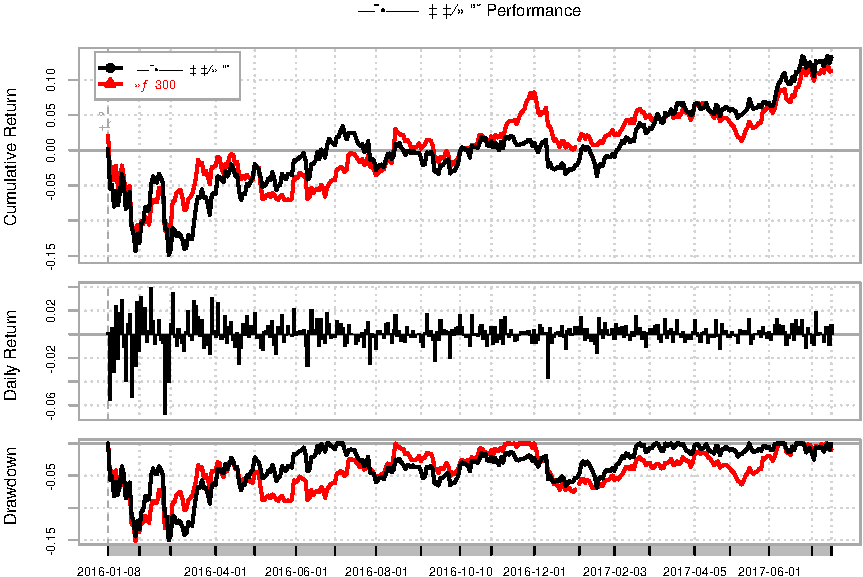
\includegraphics{wp-review_files/figure-latex/unnamed-chunk-2-1.pdf}
\caption{基金累计回报率与回撤}
\end{figure}

\begin{longtable}[]{@{}llclclc@{}}
\toprule
名称 & 最后半年 & 夏普率 & 一年 & 夏普率 & 两年 & 夏普率\tabularnewline
\midrule
\endhead
中欧行业成长混合 & 12.6\% & 2.1 & 12\% & 0.33 & 13\% &
0.25\tabularnewline
沪深300 & 8.9\% & 1.6 & 16\% & 0.28 & 11\% & 0.20\tabularnewline
\bottomrule
\end{longtable}

\begin{figure}[htbp]
\centering
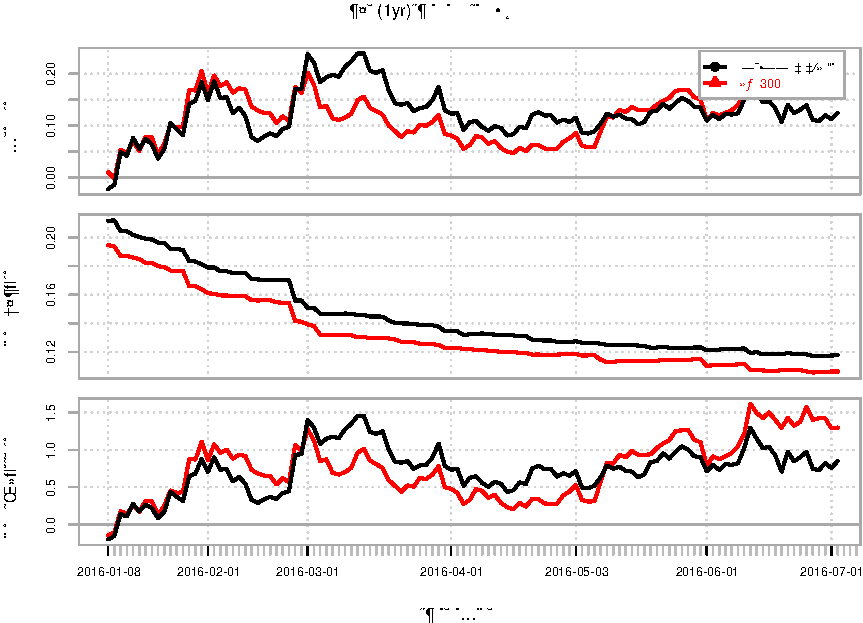
\includegraphics{wp-review_files/figure-latex/unnamed-chunk-3-1.pdf}
\caption{投资者收益风险比较}
\end{figure}

\section{简介}

复旦大学高分子物理与化学硕士。自2007年7月至2009年6月任国泰君安证券研究所助理研究员,从事化工行业分析研究工作。自2009年7月至2016年2月任银河基金管理有限公司行业研究员、基金经理助理、投资副总监兼基金经理。2016年2月加入中欧基金管理有限公司,先后担任事业部负责人、投资经理等职务。

\section{风格评述}

王培的风格集中表现为:

\begin{itemize}
\item 交易风格:多变,没有一个鲜明的主题
\item 持仓风格:早期多为小盘成长,经历转型后大盘价值,大中盘成长成为主要持仓股票
\item 主动性风格:积极主动,其主动指标达30%。
\end{itemize}

\section{\texorpdfstring{能力评价\footnote{运气能够带来超常表现,持续的好运则可以归结为能力!}}{能力评价}}

我们讲持续的超额表现归因为

\begin{equation}
\mbox{大类资产配置能力} + \mbox{行业配置能力(股票类)}+ \mbox{择股能力} + \mbox{择时能力} \Rightarrow \mbox{超额收益}
\end{equation}

\begin{table}
  \begin{tabular}{l|llll}
    因子 &大类资产配置  & 行业配置  & 择股能力 & 择时能力  \\ \hline
    贡献收益 & $0.81\%$   & $3.22\%$ & $39.40\%$ &  $-30.36\%$  \\
    评价 & 不稳定 & 弱 & 超强 & 灾难性  \\ \hline
  \end{tabular}
\end{table}

\section{投资策略简述}

\subsection{成长股精选}

\begin{itemize}
\item 将成长股的概念推广到,扩张到周期性、消费性行业等,实际上是将自己熟悉的成长股的研究方法进行推广:
\begin{itemize}
  \item 稳定增长类:以基本面投资为主;
  \item 周期类:以趋势投资为主;
  \item 阶段高成长类:主题投资为主。
  \end{itemize}
\item 寻找低估值资产和预期差:
\begin{itemize}
  \item 低估值资产是决定是否投资的关键;
  \item 预期差决定买入卖出的时点。
\end{itemize}

\end{itemize}

\subsection{风控方法}

\begin{itemize}
\item 不断衡量个股估计阶段性业绩与风格表现是否匹配来加减仓位;
\item 行业配置调整避免过高集中度;
\item 避免估值陷阱,即使估值很便宜但在基本面变差时也要及时卖出。
\end{itemize}

\section{评价}

王培是既往的成长股明星,在市场风格转变之后,经历过一段艰难转型,走向成长价值的方向上。我们基于公开信息,进行深度的科学分析,结合与其面对面的交流,做出如下评判:

\begin{enumerate}
\def\labelenumi{\arabic{enumi}.}
\tightlist
\item
  王培的交易风格不明确,甚至可以说过于频繁的操作带来了不必要的收益损失;
\item
  王培的持仓风格有从小盘成长,往大盘价值和大中盘成长转变的明确历程,深刻说明他是一位有适应能力的学习型的基金管理人,但是他的转变与继承是否能够超越市场回到他从前的高度还需要时间的验证;
\item
  作为一名``自下而上''的投资人,在大类资产配置和行业配置能力没有太出色的表现;
\item
  作为前期典型的成长股投资者和现在转型的成长价值投资这,择股能力是最为重要的盈利手段之一,王培在该项目上表现了持续有效的能力。
\end{enumerate}

因此,王培是适应多种市场风格、擅长成长类投资、积极主动的基金管理人。

\begin{acknowledgement}

在我们的分析中,使用了公开数据与部分非公开数据,在此基础上采用基于净值的风格分析,基于持仓的收益归因对基金管理人的业绩表现进行了科学的分析。我们历尽所能的使用了最为完整与详实的数据、最为科学的方法,以最为严谨的态度做出尽量客观的评价。同时我们也实地进行调研与基金经理人进行了多次的交流。在此,对于向我们提供数据与交流机会的相关人员致谢。需要根伟详细的技术分析报告,请与本文作者联系。

\end{acknowledgement}

\subsection{参考文献}
\end{document}
